% SC2001 — Chapter 8: NP-Completeness
% No document class declaration — this file is \input/\include'd by main.tex.
\chapter{NP-Completeness}
\label{ch:np}

\begin{quote}
\emph{``If P${}=$NP, the world would change profoundly; if P${}\neq$NP, we must cope.''}
NP-completeness tells us which problems admit efficient algorithms and which almost certainly do not.
\end{quote}

\noindent\textbf{Prerequisites:} Asymptotic analysis, polynomial time, reductions, and graph basics (\textsc{Vertex Cover}, \textsc{Clique}).
\section*{Learning Outcomes}
After this chapter you will be able to:
\begin{enumerate}[label=(L\arabic*)]
    \item distinguish $\mathsf{P}$, $\mathsf{NP}$, $\mathsf{coNP}$ via verifiers and certificates;
    \item define polynomial reduction and $\mathsf{NP}$-completeness (Cook--Levin) and chain reductions SAT${}\to{}$3SAT${}\to{}$\textsc{Clique}${}\to{}$\textsc{Vertex Cover};
    \item prove the $2$-approximation for \textsc{Vertex Cover} and bound greedy \textsc{Set Cover};
    \item discuss $\mathsf{P}$ vs.\ $\mathsf{NP}$ and coping strategies for $\mathsf{NP}$-complete problems.
\end{enumerate}

% ============================================================
\section{\texorpdfstring{$\mathsf{P}$, $\mathsf{NP}$, and $\mathsf{coNP}$}{P, NP, and coNP}}
\label{sec:p-np}

% --- FIND vs CHECK analogy BEFORE formal definition (with picture) ---
\begin{figure}[h]\centering
\begin{tikzpicture}[font=\small, scale=0.92]
\node[draw,rounded corners,fill=orange!10,minimum width=3.6cm,minimum height=2.2cm,align=center] (find) at (-2.6,0) {\textbf{Find} a Sudoku\\solution\\\tikz{\draw[step=0.32cm,gray] (0,0) grid (1.28,1.28);\node at (0.64,0.64){\scriptsize ?};} \\{\scriptsize search: may be exponential}};
\node[draw,rounded corners,fill=teal!10,minimum width=3.6cm,minimum height=2.2cm,align=center] (check) at (2.6,0) {\textbf{Check} a given\\solution\\\tikz{\draw[step=0.32cm,teal!40!black] (0,0) grid (1.28,1.28);\foreach \x/\y in {0.16/1.12,0.48/0.8,0.8/0.48}{\node[teal!60!black] at (\x,\y){\tiny\checkmark};}} \\{\scriptsize verify rows/cols/boxes: $O(n^2)$}};
\draw[-Latex,thick,blue!60!black] (find) -- node[above,font=\scriptsize,align=center]{hint makes\\checking easy} (check);
\end{tikzpicture}
\caption{Finding vs.\ checking. Sudoku captures $\mathsf{P}$ vs.\ $\mathsf{NP}$: \emph{finding} a solution is hard, \emph{checking} a claimed solution (certificate) is easy. $\mathsf{P}$ = can find quickly; $\mathsf{NP}$ = can check quickly given a hint.}
\label{fig:find-vs-check}
\end{figure}
Intuition first: \emph{find} vs.\ \emph{check}. Completing an empty Sudoku can take exhaustive search, but checking a filled grid is routine (scan rows, columns, boxes). NP formalises this: even if finding a proof is hard, a hint (certificate) makes verification fast. Fig.~\ref{fig:find-vs-check} is the mental model for the definitions below.

A \emph{language} $L\subseteq\{0,1\}^*$ is a decision problem: $x\in L$ means ``yes''.
We measure time in $n=|x|$ on a deterministic RAM/Turing model.

\begin{definition}[$\mathsf{P}$, informal]
$\mathsf{P}$ is the class of languages decidable by a deterministic algorithm in polynomial time, i.e.\ $O(n^c)$ for some constant $c$.
\end{definition}
Think: sorting, BFS, Dijkstra are in $\mathsf{P}$---routine even for large $n$ when $c$ is small.

\begin{definition}[$\mathsf{NP}$, verifier view]
$L\in\mathsf{NP}$ if there exists a deterministic polynomial-time \emph{verifier} $V(x,c)$ and polynomial $p$ such that $x\in L \iff \exists\, c$ with $|c|\le p(|x|)$ and $V(x,c)=1$.
The string $c$ is the \emph{certificate} (witness): it proves membership and can be checked quickly, even if finding it is hard.
\end{definition}
Equivalently, $L$ is decided by a nondeterministic machine that guesses $c$ then verifies.
Example: \textsc{3SAT} certificate is a satisfying assignment; \textsc{Clique} certificate is the $k$ vertices.
Clearly $\mathsf{P}\subseteq\mathsf{NP}$: ignore the certificate and decide directly.

\begin{remark}[$\mathsf{coNP}$]
$\mathsf{coNP}=\{\overline{L}:L\in\mathsf{NP}\}$: languages whose ``no''-answers have short certificates.
Example: \textsc{UNSAT} is in $\mathsf{coNP}$ but not known in $\mathsf{NP}$.
We have $\mathsf{P}\subseteq\mathsf{NP}\cap\mathsf{coNP}$; whether $\mathsf{NP}=\mathsf{coNP}$ is open.
\end{remark}

\begin{example}[Certificates at work]
For \textsc{Clique}$(G,k)$, list $k$ vertices; check $\binom{k}{2}$ edges in $O(n^2)$. For \textsc{Subset Sum}$(S,t)$, the subset itself. Verification is easy while search appears hard---the essence of $\mathsf{NP}$.
\end{example}

\section{\texorpdfstring{Polynomial Reductions and $\mathsf{NP}$-Completeness}{Polynomial Reductions and NP-Completeness}}
\label{sec:npc}

\begin{definition}[Polynomial reduction]
$A\le_p B$ if there is polynomial-time $f$ with $x\in A \iff f(x)\in B$ for all $x$. Intuition: $B$ is at least as hard as $A$; a solver for $B$ solves $A$ with one call plus cost of $f$.
\end{definition}

\begin{definition}[$\mathsf{NP}$-complete, $\mathsf{NP}$-hard]
$L$ is $\mathsf{NP}$-hard if every $A\in\mathsf{NP}$ satisfies $A\le_p L$.
$L$ is $\mathsf{NP}$-complete if $L\in\mathsf{NP}$ and $L$ is $\mathsf{NP}$-hard.
A polynomial algorithm for one $\mathsf{NP}$-complete problem yields one for all.
\end{definition}

\begin{theorem}[Cook--Levin, stated without proof]
\textsc{SAT} is $\mathsf{NP}$-complete.
\end{theorem}
Every $\mathsf{NP}$ verification can be encoded as a Boolean tableau whose satisfiability mirrors existence of a certificate. Since $\le_p$ is transitive, it suffices to reduce from any known $\mathsf{NP}$-complete problem.

\subsection{\texorpdfstring{SAT $\le_p$ 3SAT}{SAT <=p 3SAT}: clause splitting}
% --- GADGET before formula ---
\begin{figure}[h]\centering
\begin{tikzpicture}[font=\scriptsize, node distance=0.55cm,
  lit/.style={draw,rounded corners,fill=blue!10,minimum width=0.9cm,minimum height=0.55cm,align=center},
  aux/.style={draw,circle,fill=orange!18,minimum size=0.55cm,inner sep=0pt}]
\node[lit] (l1) {$l_1$}; \node[lit,right=of l1] (l2) {$l_2$}; \node[aux,right=of l2] (y1) {$y_1$};
\node[lit,right=of y1] (l3) {$l_3$}; \node[aux,right=of l3] (y2) {$y_2$};
\node[lit,right=of y2] (lk1) {$l_{k-1}$}; \node[lit,right=of lk1] (lk) {$l_k$};
\draw[thick,blue!50!black] (l1) -- (l2) -- (y1) -- (l3) -- (y2) -- (lk1) -- (lk);
\node[draw=none,font=\tiny,align=center,below=0.35cm of y1] {chain: fresh $y_i$ stitches long clause\\into 3-literal blocks (gadget)};
\end{tikzpicture}
\caption{SAT$\to$3SAT splitting gadget: a $k$-clause becomes $k{-}2$ clauses of size~3 using $k{-}3$ fresh variables. The gadget is satisfiable iff the original clause is.}
\label{fig:sat-3sat-gadget}
\end{figure}
A \textsc{SAT} clause $(l_1\vee\cdots\vee l_k)$ with $k>3$ is split using fresh $y_i$ (Fig.~\ref{fig:sat-3sat-gadget}):
\[
(l_1\vee l_2\vee y_1)\wedge(\bar y_1\vee l_3\vee y_2)\wedge\cdots\wedge(\bar y_{k-3}\vee l_{k-1}\vee l_k).
\]
Clauses with $1$ or $2$ literals are padded by repeating a literal. The 3-CNF is satisfiable iff the original is, and $|f(x)|=O(|x|)$. Hence SAT$\le_p$3SAT and \textsc{3SAT} is $\mathsf{NP}$-complete.

\begin{example}[Clause splitting]
$(x_1\vee\bar x_2\vee x_3\vee x_4)$ becomes $(x_1\vee\bar x_2\vee y_1)\wedge(\bar y_1\vee x_3\vee y_2)\wedge(\bar y_2\vee x_4\vee x_4)$.
\end{example}

\subsection{\texorpdfstring{3SAT $\le_p$ \textsc{Clique}}{3SAT <=p Clique}: triangles and conflicts}
% --- GADGET before formula ---
\begin{figure}[h]\centering
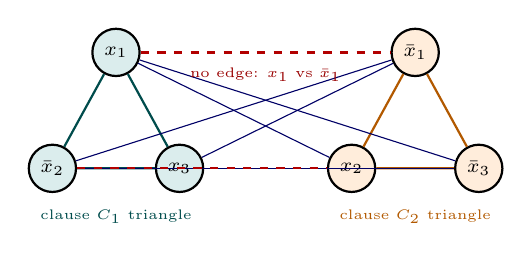
\begin{tikzpicture}[font=\scriptsize, scale=0.95,
  v/.style={circle,draw,thick,fill=blue!10,minimum size=0.6cm,inner sep=0pt}]
% two clause triangles
\node[v,fill=teal!14] (a1) at (0,1) {$x_1$}; \node[v,fill=teal!14] (a2) at (-0.85,-0.55) {$\bar x_2$}; \node[v,fill=teal!14] (a3) at (0.85,-0.55) {$x_3$};
\draw[thick,teal!60!black] (a1)--(a2)--(a3)--(a1);
\node[font=\tiny,teal!60!black] at (0,-1.2) {clause $C_1$ triangle};
\node[v,fill=orange!14] (b1) at (4,1) {$\bar x_1$}; \node[v,fill=orange!14] (b2) at (3.15,-0.55) {$x_2$}; \node[v,fill=orange!14] (b3) at (4.85,-0.55) {$\bar x_3$};
\draw[thick,orange!70!black] (b1)--(b2)--(b3)--(b1);
\node[font=\tiny,orange!70!black] at (4,-1.2) {clause $C_2$ triangle};
% compatible edges (thin), conflict omitted dashed red
\draw[thin,blue!40!black] (a1)--(b2); \draw[thin,blue!40!black] (a1)--(b3); \draw[thin,blue!40!black] (a3)--(b2);
\draw[thin,blue!40!black] (a2)--(b1); \draw[thin,blue!40!black] (a2)--(b3); \draw[thin,blue!40!black] (a3)--(b1);
\draw[dashed,red!70!black,thick] (a1)--(b1); \node[font=\tiny,red!60!black] at (2,0.7) {no edge: $x_1$ vs $\bar x_1$};
\draw[dashed,red!70!black,thick] (a2)--(b2);
\end{tikzpicture}
\caption{3SAT$\to$\textsc{Clique} gadget: one triangle per clause; connect compatible literals across clauses (omit conflict edges $x$--$\bar x$). An $m$-clique picks one literal per clause with no conflicts iff $\phi$ is satisfiable.}
\label{fig:3sat-clique-gadget}
\end{figure}
Given 3-CNF $\phi=C_1\wedge\cdots\wedge C_m$, $C_j=(\ell_{j1}\vee\ell_{j2}\vee\ell_{j3})$, build $G$ with $3m$ vertices---a triangle per clause (Fig.~\ref{fig:3sat-clique-gadget}). Connect compatible literals across clauses: add an edge between vertices in different triangles iff their literals are not complementary (i.e., not $x$ vs.\ $\bar x$). No edges within different triangles beyond that; triangle edges stay. Set $k=m$. Then $G$ has a $k$-clique iff $\phi$ is satisfiable. Size is $O(m^2)$, polynomial.

\subsection{\texorpdfstring{\textsc{Clique} $\le_p$ \textsc{Vertex Cover}}{Clique <=p Vertex Cover}: complement}
For $G=(V,E)$, $\bar G=(V,\bar E)$ is the complement. $S$ is a clique in $G$ iff $V\setminus S$ is a vertex cover in $\bar G$. So $(G,k)\mapsto(\bar G,|V|-k)$ is a reduction, and \textsc{Vertex Cover} is $\mathsf{NP}$-complete. Chaining further, \textsc{Set Cover}, \textsc{Hamiltonian Cycle}, and \textsc{Subset Sum} are also $\mathsf{NP}$-complete.

\begin{remark}[Hard vs.\ complete]
$\mathsf{NP}$-complete $\subseteq\mathsf{NP}$; $\mathsf{NP}$-hard may lie outside (e.g.\ halting, optimisation versions). Showing $L\in\mathsf{NP}$ is half the proof.
\end{remark}

% --- TIKZ 1: Reduction chain DAG ---
\begin{figure}[h]\centering
\begin{tikzpicture}[node distance=1.6cm, every node/.style={font=\small},
  box/.style={draw,thick,rounded corners,minimum width=2.2cm,minimum height=0.85cm,align=center},
  arr/.style={-Latex,thick,blue!60!black},
  arr2/.style={-Latex,thick,dashed,violet!70!black}]
\node[box,fill=blue!12] (sat) {SAT\\{\scriptsize Cook--Levin}};
\node[box,right=of sat,fill=teal!12] (3sat) {3SAT\\{\scriptsize clause split}};
\node[box,right=of 3sat,fill=orange!14] (clique) {Clique\\{\scriptsize triangles}};
\node[box,right=of clique,fill=red!10] (vc) {Vertex Cover\\{\scriptsize complement}};
\draw[arr,blue!60!black] (sat) -- node[above,font=\scriptsize,blue!60!black]{$\le_p$} (3sat);
\draw[arr,teal!60!black] (3sat) -- node[above,font=\scriptsize,teal!60!black]{$\le_p$} (clique);
\draw[arr,orange!70!black] (clique) -- node[above,font=\scriptsize,orange!70!black]{$\le_p$} (vc);
\node[draw=none,font=\scriptsize,align=center,below=0.7cm of 3sat] (etc) {$\downarrow\le_p$ Set Cover, Hamiltonian Cycle, \dots\\{\tiny each step polynomial-time; completeness propagates}};
\draw[arr2] (vc) -- (etc);
\end{tikzpicture}
\caption{Reduction chain from Cook--Levin. Hardness flows rightward.}
\label{fig:reduction-chain}
\end{figure}

% ============================================================
\section{\texorpdfstring{Coping with $\mathsf{NP}$-Completeness}{Coping with NP-Completeness}}
\label{sec:coping}
When a problem is $\mathsf{NP}$-complete we do not expect an exact polynomial algorithm: approximate, parameterise, or use heuristics.

\subsection{\texorpdfstring{$2$-approximation for \textsc{Vertex Cover}}{2-approximation for Vertex Cover} via maximal matching}
% --- maximal vs maximum picture ---
\begin{figure}[h]\centering
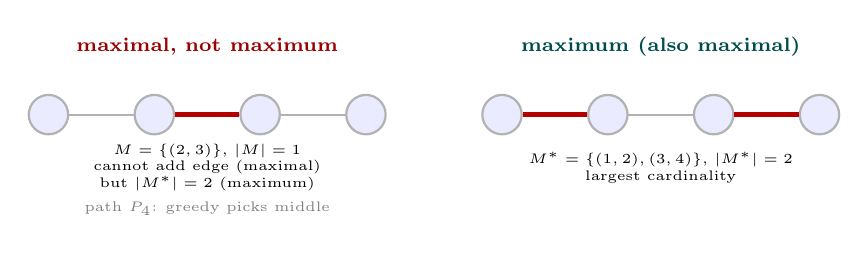
\begin{tikzpicture}[font=\scriptsize, scale=0.96,
  dot/.style={circle,draw,fill=blue!8,minimum size=0.5cm,inner sep=0pt},
  medge/.style={line width=2pt,red!70!black}, oedge/.style={thick,gray!60}]
% left: maximal but not maximum
\begin{scope}[xshift=-3.2cm]
\draw[oedge] (0,0) node[dot] (a1) {} -- (1.4,0) node[dot] (a2) {} -- (2.8,0) node[dot] (a3) {} -- (4.2,0) node[dot] (a4) {};
\draw[medge] (a2) -- (a3);
\node[draw=none,font=\scriptsize\bfseries,red!60!black] at (2.1,0.9) {maximal, not maximum};
\node[font=\tiny,align=center] at (2.1,-0.7) {$M=\{(2,3)\}$, $|M|=1$\\cannot add edge (maximal)\\but $|M^*|=2$ (maximum)};
\node[font=\tiny,gray] at (2.1,-1.25) {path $P_4$: greedy picks middle};
\end{scope}
% right: maximum
\begin{scope}[xshift=2.8cm]
\draw[oedge] (0,0) node[dot] (b1) {} -- (1.4,0) node[dot] (b2) {} -- (2.8,0) node[dot] (b3) {} -- (4.2,0) node[dot] (b4) {};
\draw[medge] (b1) -- (b2); \draw[medge] (b3) -- (b4);
\node[draw=none,font=\scriptsize\bfseries,teal!60!black] at (2.1,0.9) {maximum (also maximal)};
\node[font=\tiny,align=center] at (2.1,-0.7) {$M^*=\{(1,2),(3,4)\}$, $|M^*|=2$\\largest cardinality};
\end{scope}
\end{tikzpicture}
\caption{Maximal vs.\ maximum matching. \emph{Maximal}: cannot add any edge (local). \emph{Maximum}: largest possible (global). Approx-VC needs only maximal---any maximal matching gives the $2$-bound, no need to compute a maximum matching.}
\label{fig:maximal-vs-maximum}
\end{figure}
\textsc{Approx-VC}: pick any maximal matching $M$ (greedily add disjoint edges until stuck; Fig.~\ref{fig:maximal-vs-maximum}) and return $C$ = all endpoints of $M$.

\begin{theorem}
$C$ is a vertex cover with $|C|\le 2\cdot\textsc{OPT}$.
\end{theorem}
\emph{Proof.} $M$ maximal $\Rightarrow$ every edge shares an endpoint with some $e\in M$; thus $C$ covers all edges. Any cover needs $\ge1$ vertex per edge of $M$, disjoint $\Rightarrow \textsc{OPT}\ge|M|$. But $|C|=2|M|\le2\cdot\textsc{OPT}$. Tight on $K_{n,n}$ ($|C|=2n$, $\textsc{OPT}=n$). Time $O(n+m)$: scan edges once. Maximal $\neq$ maximum---we do not need a maximum matching (Fig.~\ref{fig:maximal-vs-maximum}).

\subsection{\texorpdfstring{Greedy \textsc{Set Cover}: $\ln n$}{Greedy Set Cover: ln n} approximation}
Repeatedly pick the set covering the most uncovered elements. Standard charging gives $|\textsc{Greedy}|\le H_n\cdot\textsc{OPT}=O(\log n)\cdot\textsc{OPT}$ where $H_n=1+\tfrac12+\cdots+\tfrac1n$, essentially optimal unless $\mathsf{P}=\mathsf{NP}$.

\subsection{Heuristic for \textsc{TSP}: nearest neighbour}
Start at any city, go to nearest unvisited city, return. No constant-factor guarantee for general TSP (unless $\mathsf{P}=\mathsf{NP}$); on metric instances it can be $\Theta(\log n)$ off, but $O(n^2)$ and often reasonable. Better guarantees need Christofides ($1.5$-approx on metric TSP).

% --- TIKZ 2: P vs NP Venn ---
\begin{figure}[h]\centering
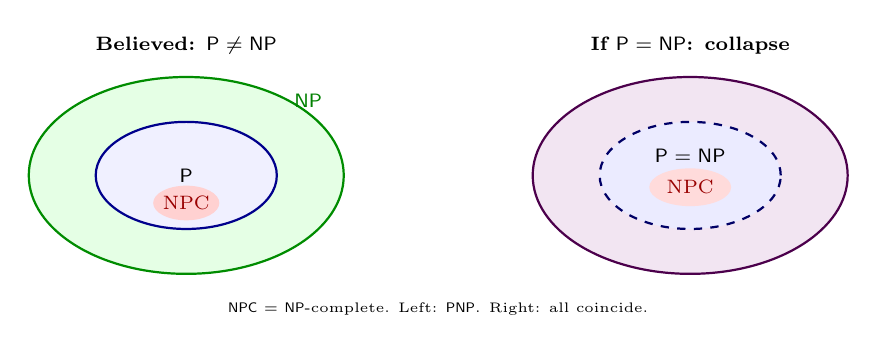
\begin{tikzpicture}[font=\small]
\begin{scope}[xshift=-3.2cm]
  \fill[green!10] (0,0) ellipse (2.0 and 1.25);
  \fill[blue!6] (0,0) ellipse (1.15 and 0.68);
  \draw[thick,green!55!black] (0,0) ellipse (2.0 and 1.25);
  \draw[thick,blue!55!black] (0,0) ellipse (1.15 and 0.68);
  \fill[red!18] (0,-0.35) ellipse (0.42 and 0.22);
  \node[font=\scriptsize,align=center] at (0,0) {$\mathsf{P}$};
  \node[font=\scriptsize,green!50!black] at (1.55,0.95) {$\mathsf{NP}$};
  \node[font=\scriptsize,align=center,red!60!black] at (0,-0.35) {NPC};
  \node[draw=none,font=\scriptsize\bfseries] at (0,1.65) {Believed: $\mathsf{P}\neq\mathsf{NP}$};
\end{scope}
\begin{scope}[xshift=3.2cm]
  \fill[violet!10] (0,0) ellipse (2.0 and 1.25);
  \fill[blue!8] (0,0) ellipse (1.15 and 0.68);
  \fill[red!14] (0,-0.15) ellipse (0.52 and 0.24);
  \draw[thick,violet!60!black] (0,0) ellipse (2.0 and 1.25);
  \draw[thick,blue!40!black,dashed] (0,0) ellipse (1.15 and 0.68);
  \node[font=\scriptsize,align=center] at (0,0.25) {$\mathsf{P}=\mathsf{NP}$};
  \node[font=\scriptsize,red!60!black] at (0,-0.15) {NPC};
  \node[draw=none,font=\scriptsize\bfseries] at (0,1.65) {If $\mathsf{P}=\mathsf{NP}$: collapse};
\end{scope}
\node[draw=none,font=\tiny,align=center] at (0,-1.7) {$\mathsf{NPC}$ = $\mathsf{NP}$-complete. Left: $\mathsf{P}\subsetneq\mathsf{NP}$. Right: all coincide.};
\end{tikzpicture}
\caption{Two views of $\mathsf{P}$ vs.\ $\mathsf{NP}$. Left is widely believed; right would make every $\mathsf{NP}$ problem tractable.}
\label{fig:p-np-venn}
\end{figure}

\section{\texorpdfstring{$\mathsf{P}$ vs.\ $\mathsf{NP}$ and Why $\mathsf{P}\neq\mathsf{NP}$ Is Believed}{P vs. NP and Why P != NP Is Believed}}
\label{sec:p-vs-np}
$\mathsf{P}$ vs.\ $\mathsf{NP}$ asks whether every efficiently verifiable problem is efficiently solvable. $\mathsf{P}=\mathsf{NP}$ would give polynomial algorithms for all $\mathsf{NP}$-complete problems (cryptography breaks); $\mathsf{P}\neq\mathsf{NP}$ confirms hardness. Evidence for $\mathsf{P}\neq\mathsf{NP}$: decades of failed search, oracle/barrier results, and cryptographic practice that would otherwise collapse. A polynomial algorithm for any $\mathsf{NP}$-complete problem propagates via $\le_p$ to all of $\mathsf{NP}$ (Fig.~\ref{fig:reduction-chain}). Belief is not proof---separation must rule out \emph{all} polynomial algorithms.

\paragraph{Reduction size check.} Each construction is polynomial: SAT~$\to$~3SAT blows $k$-clause into $k{-}2$ clauses with $k{-}3$ fresh variables; 3SAT~$\to$~\textsc{Clique} creates $3m$ vertices, $O(m^2)$ edges; \textsc{Clique}~$\to$~\textsc{Vertex Cover} complements in $O(n^2)$.

\section{Chapter Notes}
Cook (1971) and Levin (1973) founded $\mathsf{NP}$-completeness; Karp (1972) listed 21 reductions. Garey--Johnson remains the catalogue. CLRS Ch.~34 is concise; Sipser Ch.~7 gives the language view; Arora--Barak Ch.~2 covers Cook--Levin. Exam tip: to prove $X$ $\mathsf{NP}$-complete, show (a) $X\in\mathsf{NP}$ (verifier) and (b) $Y\le_p X$ for known $\mathsf{NP}$-complete $Y$.

% ============================================================
\section{Exercises}
\label{sec:ch08-exercises}

\begin{exercise}[Certificate vs.\ decision]
Give verifiers for \textsc{Subset Sum} and \textsc{Hamiltonian Cycle} to show each is in $\mathsf{NP}$. Why is the complement not obviously in $\mathsf{NP}$ (what about $\mathsf{coNP}$)?
\end{exercise}

\begin{exercise}[Reductions by hand]
(a) Convert $\phi=(x_1\vee x_2)\wedge(\bar x_1\vee\bar x_2\vee x_3)\wedge(x_1\vee\bar x_3\vee x_4\vee\bar x_5)$ to 3-CNF via clause splitting; count new variables/clauses. (b) Apply 3SAT$\to$\textsc{Clique} to your 3-CNF and draw $G$; identify the $m$-clique for $x_1=1,x_2=0,x_3=1$. (c) Exhibit the complementary vertex cover.
\end{exercise}

\begin{exercise}[Approximation analysis]
(a) Show $2$-approx for \textsc{Approx-VC} is tight ($|C|=2\cdot\textsc{OPT}$ family). (b) Show greedy \textsc{Set Cover} achieves $H_n$ by charging $1/k$. (c) Give $4$-city TSP where nearest-neighbour is $>2\times$ optimal; why no constant factor for general TSP unless $\mathsf{P}=\mathsf{NP}$?
\end{exercise}

\begin{exercise}[$\mathsf{P}$ vs.\ $\mathsf{NP}$ consequences]
Assume $\mathsf{P}=\mathsf{NP}$. (a) Show every $\mathsf{NP}$-complete language is in $\mathsf{P}$ and outline solving \textsc{3SAT} in polynomial time. (b) Why would factoring-based crypto be at risk even though factoring is not known $\mathsf{NP}$-complete? (c) If $\mathsf{NP}\neq\mathsf{coNP}$, what about $\mathsf{P}$ vs.\ $\mathsf{NP}$?
\end{exercise}
% End of Chapter 8
